% Line Atlas chapter draft.
% Suggested dependencies: amsmath, amssymb, bm, siunitx, booktabs,
% tabularx, tikz, pgfplots, xcolor, hyperref. Set \pgfplotsset{compat=1.18}.
% Citation keys are defined in line_atlas_references.bib.

\chapter{Radiation, Matter, and the Making of a Spectral Line}
\label{chap:radiative-transfer-foundations}
\chaptermark{Radiation, Matter, and Spectral Lines}

Spectral lines are not labels pasted onto otherwise featureless spectra.  They are
the observable end point of a chain of physical events: particles are placed in
quantum states, photons are created or destroyed, radiation propagates through a
structured medium, and an instrument averages the emerging field over angle,
wavelength, and time.  A line atlas is most useful when every entry can be read in
both directions along this chain.  From an observed feature one would like to infer
density, temperature, abundance, velocity, and radiation field; from a proposed
physical model one would like to predict a measurable flux profile.

This chapter establishes the vocabulary needed for both directions.  It emphasizes
the assumptions hidden in familiar formulae and the combinations of quantities that
spectra actually constrain.  More complete treatments are given by
\citet{RybickiLightman1979}, \citet{Mihalas1978},
\citet{OsterbrockFerland2006}, and \citet{Draine2011}.

\section{What a spectrograph measures}

The fundamental radiometric quantity is the specific intensity
$I_\nu(\boldsymbol{x},\hat{\boldsymbol{n}},t)$, defined so that the energy crossing an
area element $\mathrm{d}A$ in time $\mathrm{d}t$, within solid angle
$\mathrm{d}\Omega$ and frequency interval $\mathrm{d}\nu$, is
\begin{equation}
 \mathrm{d}E = I_\nu\cos\theta\,\mathrm{d}A\,\mathrm{d}t\,
              \mathrm{d}\Omega\,\mathrm{d}\nu .
 \label{eq:rt-intensity-definition}
\end{equation}
Unlike flux, intensity is conserved along a ray in empty Euclidean space.  The
monochromatic flux is the first angular moment,
\begin{equation}
 F_\nu = \int_{4\pi} I_\nu(\hat{\boldsymbol{n}})\cos\theta\,\mathrm{d}\Omega ,
 \qquad
 J_\nu = \frac{1}{4\pi}\int_{4\pi}I_\nu\,\mathrm{d}\Omega ,
 \label{eq:rt-moments}
\end{equation}
where $J_\nu$ is the mean intensity.  An unresolved source at luminosity distance
$D_L$ is normally reported through a flux density $f_\nu$ or $f_\lambda$.  The two
are not numerically interchangeable:
\begin{equation}
 f_\lambda = f_\nu\left|\frac{\mathrm{d}\nu}{\mathrm{d}\lambda}\right|
 = f_\nu\frac{c}{\lambda^2},
 \qquad \lambda f_\lambda=\nu f_\nu .
 \label{eq:fnu-flambda}
\end{equation}
This Jacobian is the reason that a spectrum flat in $f_\nu$ slopes as
$\lambda^{-2}$ in $f_\lambda$.

For a source at redshift $z$, $\nu_{\rm obs}=\nu_{\rm em}/(1+z)$ and
$\lambda_{\rm obs}=(1+z)\lambda_{\rm em}$.  Specific intensity obeys the
Liouville invariant $I_\nu/\nu^3$ along a null geodesic in the absence of
interactions.  Consequently surface brightness dims as $(1+z)^{-4}$ after
integrating over frequency.  Line luminosity and observed integrated line flux are
related by
\begin{equation}
 F_{\rm line}=\int f_\lambda\,\mathrm{d}\lambda_{\rm obs}
             =\frac{L_{\rm line}}{4\pi D_L^2}.
 \label{eq:line-flux-luminosity}
\end{equation}
No extra factor of $(1+z)$ belongs in this bolometric line relation; such factors
enter relations between spectral densities or between velocity-integrated radio
brightness and luminosity.

\paragraph{Definition: line profile.}
The line profile $\phi(\nu)$ is a probability density in frequency, normalized as
$\int\phi(\nu)\,\mathrm{d}\nu=1$.  It therefore has units of inverse frequency.
Omitting this unit is a common route to dimensionally incorrect opacity formulae.

\section{The transfer equation and its formal solution}

Along path length $s$, emission adds radiation and extinction removes it:
\begin{equation}
 \frac{\mathrm{d}I_\nu}{\mathrm{d}s}=j_\nu-\alpha_\nu I_\nu,
 \label{eq:transfer-dimensional}
\end{equation}
where $j_\nu$ is the emission coefficient per steradian and $\alpha_\nu$ is the
extinction coefficient.  True absorption and scattering may both contribute to
$\alpha_\nu$; only true absorption transfers radiant energy to internal energy.
Define optical depth increasing away from the observer by
$\mathrm{d}\tau_\nu=\alpha_\nu\mathrm{d}s$ and source function
$S_\nu=j_\nu/\alpha_\nu$.  For a slab of total optical depth $\tau_\nu$, the
emergent intensity is
\begin{equation}
 I_\nu(0)=I_\nu(\tau_\nu)e^{-\tau_\nu}
 +\int_0^{\tau_\nu} S_\nu(t)e^{-t}\,\mathrm{d}t .
 \label{eq:formal-solution}
\end{equation}
For a homogeneous slab this becomes
\begin{equation}
 I_{\nu,\rm out}=I_{\nu,\rm bg}e^{-\tau_\nu}
                 +S_\nu\left(1-e^{-\tau_\nu}\right).
 \label{eq:homogeneous-slab}
\end{equation}
Equation~\eqref{eq:homogeneous-slab} is one of the most useful diagnostic equations
in spectroscopy.  A feature appears in emission when the line source function
exceeds the incident background intensity and in absorption when it is smaller.
Thus ``emission line'' and ``absorption line'' describe contrast, not an intrinsic
property of a transition.

When the material is in local thermodynamic equilibrium (LTE), detailed balance
gives $S_\nu=B_\nu(T)$, the Planck function.  LTE requires collisional processes to
establish local level populations, but does not require the radiation field to be a
blackbody.  In a stratified, optically thick atmosphere with a slowly varying source
function, the Eddington--Barbier approximation gives
$I_\nu(0,\mu)\simeq S_\nu(\tau_\nu=\mu)$, where
$\mu=\cos\theta$.  We therefore see different physical depths at different
frequencies: high-opacity line cores form closer to the surface than adjacent
continuum.

\subsection{Absorption, stimulated emission, and spontaneous emission}

Consider lower and upper states $l$ and $u$, populations $n_l$ and $n_u$, and
statistical weights $g_l$ and $g_u$.  Einstein coefficients describe absorption
($B_{lu}$), stimulated emission ($B_{ul}$), and spontaneous emission ($A_{ul}$).
Their thermodynamic relations are
\begin{equation}
 g_lB_{lu}=g_uB_{ul},\qquad
 A_{ul}=\frac{2h\nu_0^3}{c^2}B_{ul}.
 \label{eq:einstein-relations}
\end{equation}
For complete redistribution with the same normalized line profile for absorption
and emission,
\begin{align}
 j_\nu^{\rm line} &= \frac{h\nu_0}{4\pi}n_uA_{ul}\phi(\nu),\\
 \alpha_\nu^{\rm line} &= \frac{h\nu_0}{4\pi}
             \left(n_lB_{lu}-n_uB_{ul}\right)\phi(\nu).
 \label{eq:line-j-alpha}
\end{align}
The negative stimulated-emission term matters at radio wavelengths and in population
inversions.  It should not be silently discarded merely because spontaneous emission
dominates a particular optical application.

The absorption oscillator strength $f_{lu}$ is related to the frequency-integrated
cross section by
\begin{equation}
 \int\sigma_\nu\,\mathrm{d}\nu=\frac{\pi e^2}{m_ec}f_{lu},
 \qquad
 \sigma_\nu=\frac{\pi e^2}{m_ec}f_{lu}\phi(\nu).
 \label{eq:oscillator-strength-cross-section}
\end{equation}
Oscillator strengths are dimensionless atomic data.  Their uncertainty can dominate
an abundance measurement even when the spectrum has extremely high signal-to-noise.

\section{Population equations: LTE and statistical equilibrium}

In LTE, excitation follows the Boltzmann relation,
\begin{equation}
 \frac{n_u}{n_l}=\frac{g_u}{g_l}
 \exp\!\left[-\frac{E_u-E_l}{kT}\right],
 \label{eq:boltzmann-populations}
\end{equation}
and adjacent ionization stages follow the Saha equation,
\begin{equation}
 \frac{n_{i+1}n_e}{n_i}=
 \frac{2}{\lambda_e^3}\frac{U_{i+1}(T)}{U_i(T)}
 \exp\!\left(-\frac{\chi_i}{kT}\right),
 \qquad
 \lambda_e=\frac{h}{\sqrt{2\pi m_ekT}}.
 \label{eq:saha}
\end{equation}
Here $U_i$ is a partition function and $\chi_i$ the ionization potential.  Nebulae,
diffuse clouds, and the circumgalactic medium are generally not in LTE.  Their level
populations instead satisfy statistical equilibrium,
\begin{equation}
 \sum_{j\ne i}n_jP_{ji}=n_i\sum_{j\ne i}P_{ij},
 \qquad \sum_i n_i=n_{\rm species},
 \label{eq:statistical-equilibrium}
\end{equation}
where each $P_{ij}$ may contain radiative, electron-impact, neutral-impact,
recombination, charge-exchange, or chemical rates.

For an optically thin two-level ion excited by electron collisions, neglecting
stimulated terms,
\begin{equation}
 \frac{n_u}{n_l}=\frac{n_eq_{lu}}{A_{ul}+n_eq_{ul}},
 \qquad n_{\rm crit}=\frac{A_{ul}}{q_{ul}}.
 \label{eq:two-level-atom}
\end{equation}
At $n_e\ll n_{\rm crit}$, each excitation is usually followed by a photon, so the
volume emissivity scales approximately as $n_en_l$.  At
$n_e\gg n_{\rm crit}$, collisions de-excite the upper state and the line no longer
grows quadratically.  For a multilevel atom the denominator must include every
downward collider and radiative branch,
\begin{equation}
 n_{{\rm crit},u}=\frac{\sum_{l<u}A_{ul}}
 {\sum_{j\ne u}\sum_c n_cq^{(c)}_{uj}/n_e},
 \label{eq:multilevel-critical-density}
\end{equation}
or, more transparently, one quotes a collider-specific critical density
$n_{{\rm crit},c}=\sum A_{ul}/\sum q^{(c)}_{uj}$.  Tabulated critical densities are
therefore temperature dependent and are not universal constants of a line.

\paragraph{Caveat: critical density is not a hard boundary.}
Line emissivity changes smoothly around $n_{\rm crit}$.  Radiative trapping lowers
the effective spontaneous escape rate, while continuum pumping raises levels without
collisions.  A measured density-sensitive ratio should be interpreted with a full
multilevel model when optical depth, fluorescence, or several colliders matter.

\section{Why lines have width and shape}

The natural profile of an isolated damped transition is Lorentzian.  Thermal and
microturbulent Doppler shifts produce a Gaussian core.  Their convolution is the
Voigt profile,
\begin{equation}
 \phi(\nu)=\frac{H(a,u)}{\sqrt{\pi}\Delta\nu_D},\quad
 u=\frac{\nu-\nu_0}{\Delta\nu_D},\quad
 a=\frac{\Gamma}{4\pi\Delta\nu_D},
 \label{eq:voigt-profile}
\end{equation}
where $\Gamma$ is the total damping rate and
\begin{equation}
 \Delta\nu_D=\frac{\nu_0b}{c},\qquad
 b^2=\frac{2kT}{m}+b_{\rm nt}^2.
 \label{eq:doppler-b}
\end{equation}
The Doppler parameter $b$ is related to a Gaussian velocity dispersion by
$b=\sqrt{2}\sigma_v$ and to full width at half maximum by
$\mathrm{FWHM}=2\sqrt{\ln2}\,b\simeq1.665b$.  Mixing these conventions can bias
temperatures by a factor of two.

If two ions share the same temperature and nonthermal broadening, their measured
widths obey
\begin{equation}
 b_1^2-b_2^2=2kT\left(\frac{1}{m_1}-\frac{1}{m_2}\right).
 \label{eq:two-ion-temperature}
\end{equation}
The method is powerful only when the profiles are demonstrably co-spatial and the
instrumental line-spread function has been removed.  Unresolved component structure
usually mimics nonthermal broadening.

\begin{figure}[tbp]
\centering
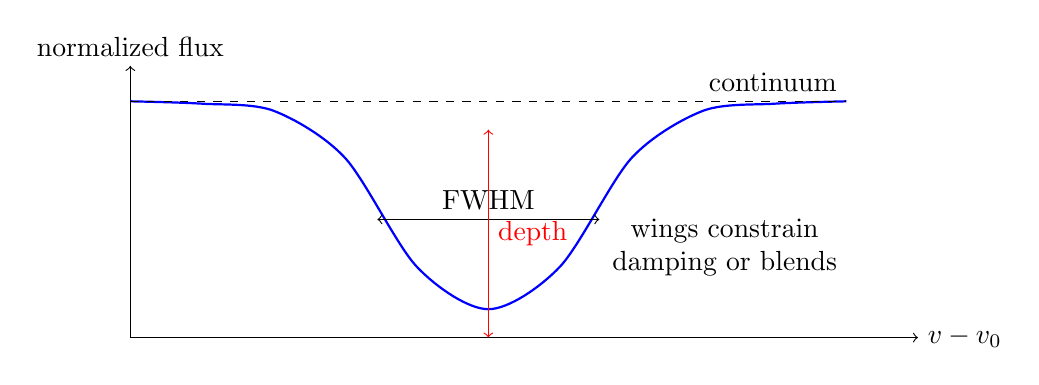
\begin{tikzpicture}[x=0.075\linewidth,y=3.0cm]
  \draw[->] (0,0) -- (11,0) node[right] {$v-v_0$};
  \draw[->] (0,0) -- (0,1.15) node[above] {normalized flux};
  \draw[thick,blue]
    plot[smooth] coordinates {(0,1.0) (1,0.99) (2,0.96) (3,0.76)
    (4,0.30) (5,0.12) (6,0.30) (7,0.76) (8,0.96) (9,0.99) (10,1.0)};
  \draw[dashed] (0,1) -- (10,1) node[above left] {continuum};
  \draw[<->] (3.45,0.50) -- (6.55,0.50)
    node[midway,above] {FWHM};
  \draw[<->,red] (5,0) -- (5,0.88)
    node[midway,right] {depth};
  \node[align=center] at (8.3,0.38) {wings constrain\\damping or blends};
\end{tikzpicture}
\caption{Original schematic for a normalized absorption profile.  A production
version can overlay intrinsic, instrument-convolved, and sampled profiles.  The
equivalent width is the area between the continuum and profile, not simply depth
times FWHM.}
\label{fig:line-profile-anatomy}
\end{figure}

Macroscopic velocity gradients produce profiles that cannot be represented by a
single Voigt function.  Rotation can create a double-horned integrated profile;
accelerating outflows can form P-Cygni profiles; self-absorption can split an
otherwise single emission peak.  The measured spectrum is finally convolved with
the instrument line-spread function $L$ and integrated over detector pixels:
\begin{equation}
 f_i=\int_{\Delta\lambda_i}
       \left[f_{\lambda,\rm true}*L\right](\lambda)\,
       R_i(\lambda)\,\mathrm{d}\lambda,
 \label{eq:forward-instrument}
\end{equation}
where $R_i$ includes pixel response.  Deconvolving noisy data is unstable; forward
convolution of a physical model is normally preferable.

\section{Optical depth, equivalent width, and the curve of growth}

For a column density $N_l$ in the lower state, a Doppler-broadened absorption line
has central optical depth
\begin{equation}
 \tau_0=\frac{\sqrt{\pi}e^2}{m_ec}
         \frac{f_{lu}\lambda_0N_l}{b}
 =1.497\times10^{-15}
 \frac{N_l}{\mathrm{cm}^{-2}}
 \frac{f_{lu}(\lambda_0/\text{\AA})}{b/(\mathrm{km\,s^{-1}})}.
 \label{eq:line-center-optical-depth}
\end{equation}
The rest-frame equivalent width of an absorption line is
\begin{equation}
 W_0=\int\left(1-\frac{F_\lambda}{F_c}\right)
      \mathrm{d}\lambda_{\rm rest},
 \qquad W_{\rm obs}=(1+z)W_0.
 \label{eq:equivalent-width}
\end{equation}
For optically thin absorption,
\begin{equation}
 W_0=\frac{\pi e^2}{m_ec^2}N_lf_{lu}\lambda_0^2,
 \label{eq:linear-cog}
\end{equation}
independent of $b$.  As the core saturates, increasing $N_l$ mostly broadens the
black portion of the line and $W$ grows only roughly as $b\sqrt{\ln \tau_0}$.
At still larger columns, Lorentzian damping wings cause
$W\propto N_l^{1/2}$.  These are the linear, saturated, and damping regimes of the
curve of growth.

\begin{figure}[tbp]
\centering
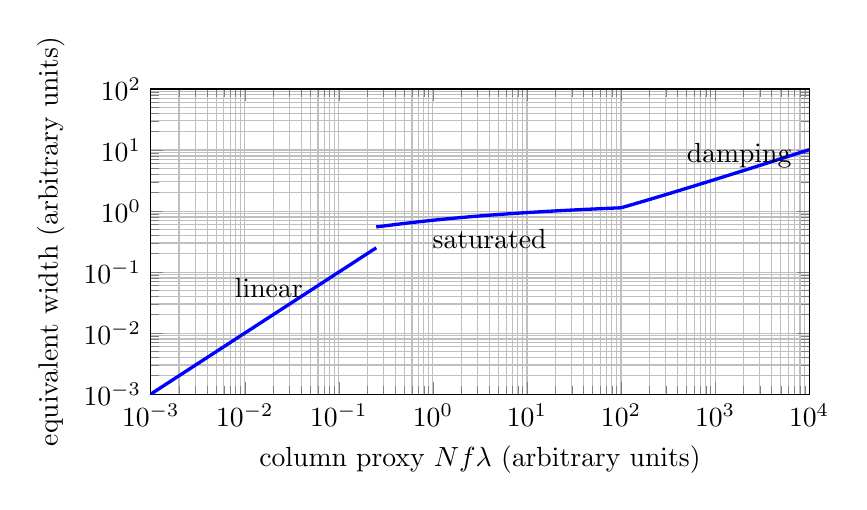
\begin{tikzpicture}
\begin{loglogaxis}[
 width=0.82\linewidth,height=0.45\linewidth,
 xlabel={column proxy $Nf\lambda$ (arbitrary units)},
 ylabel={equivalent width (arbitrary units)},
 xmin=1e-3,xmax=1e4,ymin=1e-3,ymax=1e2,
 grid=both,legend style={draw=none,fill=none},
]
 \addplot[very thick,blue,domain=0.001:0.25,samples=40] {x};
 \addplot[very thick,blue,domain=0.25:100,samples=80]
   {0.25+0.36*sqrt(ln(1+4*x))};
 \addplot[very thick,blue,domain=100:10000,samples=60]
   {0.25+0.36*sqrt(ln(401))+0.10*(sqrt(x)-10)};
 \node at (axis cs:0.018,0.055) {linear};
 \node at (axis cs:4,0.35) {saturated};
 \node at (axis cs:1800,8) {damping};
\end{loglogaxis}
\end{tikzpicture}
\caption{Pedagogical curve-of-growth concept generated entirely with PGFPlots.
The plotted interpolation is schematic, not a substitute for evaluating a Voigt
profile.  A final atlas could add families of curves for several Doppler parameters.}
\label{fig:curve-of-growth-concept}
\end{figure}

\subsection{Worked example: is a Ly\texorpdfstring{$\alpha$}{-alpha} absorber optically thin?}

Take H\,I Ly$\alpha$ with $f=0.4164$ and
$\lambda_0=1215.67$~\AA.  For
$N_{\mathrm{H\,I}}=10^{14}\,\mathrm{cm}^{-2}$ and
$b=20\,\mathrm{km\,s^{-1}}$, equation~\eqref{eq:line-center-optical-depth}
gives
\begin{equation}
 \tau_0\simeq1.497\times10^{-15}
 \frac{10^{14}\times0.4164\times1215.67}{20}\simeq3.8.
\end{equation}
The line is already saturated at its center, even though its neutral-hydrogen column
is modest by interstellar standards.  Applying the optically thin equivalent-width
formula would underestimate $N_{\mathrm{H\,I}}$.  Higher Lyman-series transitions,
a curve-of-growth analysis, or a forward Voigt-profile fit are needed.  A formally
excellent single-component fit can still be wrong if narrow components are hidden by
the line-spread function.

\section{Emission measure, surface brightness, and luminosity}

For optically thin recombination radiation, the line emissivity integrated over
solid angle is often written
\begin{equation}
 \epsilon_{ul}=h\nu_{ul}n_en_{i+1}\alpha^{\rm eff}_{ul}(T),
 \qquad
 L_{ul}=\int_V\epsilon_{ul}\,\mathrm{d}V.
 \label{eq:recombination-emissivity}
\end{equation}
The effective recombination coefficient includes cascades that feed the upper state.
The surface brightness scales with emission measure,
\begin{equation}
 {\rm EM}=\int n_en_p\,\mathrm{d}\ell,
 \qquad
 I_{ul}=\frac{h\nu_{ul}}{4\pi}
 \int n_en_p\alpha^{\rm eff}_{ul}(T)\,\mathrm{d}\ell.
 \label{eq:emission-measure}
\end{equation}
Because EM weights density squared, dense clumps dominate emission.  Absorption
columns weight density linearly.  Combining emission and absorption is therefore a
way to constrain clumping, but only if the two measurements sample the same gas.

Collisionally excited forbidden lines have low-density emissivity
\begin{equation}
 \epsilon_{ul}\simeq n_en(X^i)q_{lu}(T)h\nu_{ul}
 \frac{A_{ul}}{\sum_k A_{uk}},
 \label{eq:cel-emissivity}
\end{equation}
with excitation coefficient
\begin{equation}
 q_{lu}(T)=\frac{8.629\times10^{-6}}{g_lT^{1/2}}
 \Upsilon_{lu}(T)\exp\!\left(-\frac{\Delta E}{kT}\right)
 \quad \mathrm{cm^3\,s^{-1}}.
 \label{eq:collisional-rate-coefficient}
\end{equation}
The effective collision strength $\Upsilon$ varies more gently with temperature
than the exponential.  This strong temperature sensitivity makes auroral-to-nebular
ratios valuable thermometers and also makes inferred abundances sensitive to
unresolved temperature structure.

\subsection{Worked example: a density-sensitive doublet}

Suppose two lines arise from metastable levels with different $A/q$ values but close
excitation energies.  Their ratio can be approximated schematically by
\begin{equation}
 R(n_e)=R_0\frac{1+n_e/n_{{\rm crit},2}}
                     {1+n_e/n_{{\rm crit},1}}.
 \label{eq:doublet-density-schematic}
\end{equation}
At densities below both critical densities, $R\rightarrow R_0$ and the diagnostic
loses leverage.  At densities above both, it approaches another asymptote and again
loses leverage.  The ratio is informative primarily between the two critical
densities.  An observer should report an upper or lower limit when a measured ratio
lies near an asymptote, rather than quote a spuriously precise density.

\section{Resonant scattering, escape, and redistribution}

Resonance lines such as Ly$\alpha$, C\,IV, Mg\,II, and Na\,I D may scatter many
times before escape.  Scattering conserves photon number only in the idealized
absence of dust absorption, collisional de-excitation, conversion to other lines, or
escape outside the aperture.  A simple escape-probability approximation replaces
$A_{ul}$ by $\beta(\tau)A_{ul}$, where for a static slab one rough choice is
\begin{equation}
 \beta(\tau)\simeq\frac{1-e^{-\tau}}{\tau}.
 \label{eq:escape-probability}
\end{equation}
This captures the limiting trends but not detailed frequency diffusion or geometry.
At large optical depth, photons escape through frequency excursions into the wings;
bulk velocity and dust geometry can then shape the emergent profile more strongly
than the intrinsic production spectrum.

\paragraph{Interpretive caution.}
The centroid of a resonant emission line need not equal the systemic velocity, and
its integrated flux need not measure only the production rate.  A spatially extended
halo may be composed largely of photons created in the central region and scattered
into the line of sight.  Conversely, a narrow spectroscopic aperture may classify
scattered photons as ``destroyed'' even when they merely emerge elsewhere.

\section{A hierarchy of modeling assumptions}

Line interpretation should state its rung on the following hierarchy:
\begin{enumerate}
 \item \textbf{Optically thin emissivity or absorption.}  Photons interact at most
 once; geometry enters only through an integral of density or density squared.
 \item \textbf{One-zone statistical equilibrium.}  Level populations respond to a
 specified temperature, density, radiation field, and abundance pattern.
 \item \textbf{Photoionization or shock structure.}  Thermal balance, ionization,
 chemistry, and attenuation vary through the source.
 \item \textbf{Radiative transfer in prescribed geometry.}  Optical depth,
 scattering, and velocity fields determine escape.
 \item \textbf{Radiation hydrodynamics or magnetohydrodynamics.}  Radiation changes
 the gas whose structure in turn changes the radiation.
\end{enumerate}
Increasing sophistication does not automatically improve inference.  A complex
model with unconstrained geometry can be less informative than a transparent
line-ratio estimate.  The minimum adequate model is the simplest rung that includes
all processes capable of shifting the desired quantity by more than the error budget.

\section{Checklist for a trustworthy line interpretation}

Before assigning a physical meaning to a feature, ask:
\begin{itemize}
 \item Is the wavelength in vacuum or air, and is the velocity convention stated?
 \item Is the line resolved relative to the full, possibly non-Gaussian,
 line-spread function?
 \item Is the continuum model flexible enough, but not so flexible that it absorbs
 broad wings?
 \item Can a second transition reveal saturation, blending, fluorescence, or
 density sensitivity?
 \item Are LTE, optical thinness, equilibrium, and a single temperature justified?
 \item Does the aperture include all scattered or diffuse emission relevant to the
 physical question?
 \item Which atomic data set supplies wavelengths, $A$ values, collision strengths,
 and oscillator strengths, and are their uncertainties propagated?
 \item Does the quoted uncertainty include calibration, model discrepancy, and
 component degeneracy in addition to photon noise?
\end{itemize}

The rest of the atlas repeatedly returns to these questions.  A transition becomes
a diagnostic only after its population mechanism, transfer regime, and measurement
operator have been specified.
